本章主要用于测试该模版。

\subsection{图片}
图\ref{f1}为FPGA基本单元结构图。
\begin{figure}[H] % H为当前位置,!htb为忽略美学标准,htbp为浮动图形
    \centering
    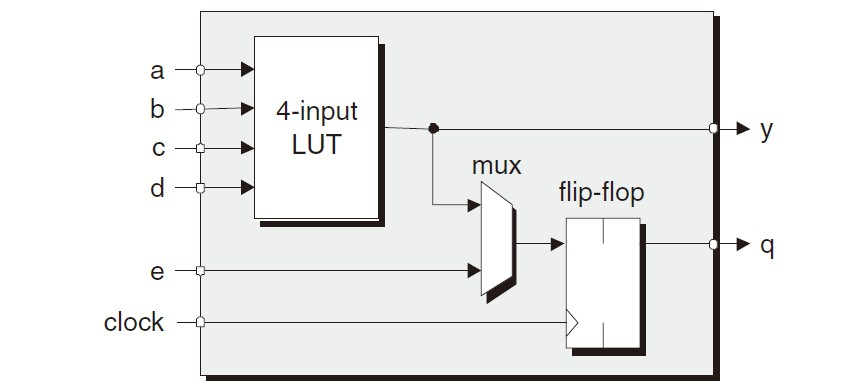
\includegraphics{img/FPGA.jpg} % option中可以用scale缩放,用height和width指定长宽
    \caption{Slice of FPGA} %最终文档中希望显示的图片标题
    \label{f1} %用于文内引用的标签
\end{figure}

FPGA的基本单元是Slice,主要包括LUT、MUX及触发器,其中每个Slice的大小和FPGA型号有关。

\subsection{表格}
表\ref{t1}使用Excel2LaTeX自动生成。

% Table generated by Excel2LaTeX from sheet 'Sheet1'
\begin{table}[htbp]
    \centering
    \caption{使用Excel2LaTeX}
      \begin{tabular}{|c|ccc|}
        \hline
        date  & data1 & data2 & sum \\
        1     & 1     & 1     & 2 \\
        2     & 2     & 2     & 4 \\
        3     & 3     & 3     & 6 \\
        4     & 4     & 4     & 8 \\
        5     & 5     & 5     & 10 \\
        6     & 6     & 6     & 12 \\
        7     & 7     & 7     & 14 \\
        8     & 8     & 8     & 16 \\
        9     & 9     & 9     & 18 \\
        \hline
      \end{tabular}%
    \label{t1}%
\end{table}%
  
表\ref{t2}手动绘制。

\begin{table}[htbp]
    \centering
    \caption{手动绘制}
    \begin{tabular}{|l|ccc|}
        \hline
        \diagbox{Time}{Room}{Day} & Mon & Tue & Wed \\
        \hline
        Morning & used & used & \\
        Afternoon & & used & used \\
        \hline
    \end{tabular}
    \label{t2}%
\end{table}%

\subsection{数学}
这里有一个数学公式
\begin{equation}
    \int_1^2 x dx = \frac{3}{2} 
\end{equation}

\subsubsection{数学公式说明}
这是一个简单的积分.

\subsection{代码}
推荐的verilog代码风格如下所示,但目前空格对齐的方式还没完全理解清楚。
\lstset{language=verilog}
\begin{lstlisting}
    module clk_div # (
        parameter   DIV    = 434 // BPS = 50M/434 = 115200    
    )(
        input       clk_in,
        input       rst_n,
        output reg  clk_out
    );
    
    reg  [12 : 0] cnt;
    wire [12 : 0] cnt_nxt = cnt + 1'b1;
    always @ (posedge clk_in or negedge rst_n) begin
        if (~rst_n) cnt <= 13'b0;
        else if (cnt < DIV) cnt <= cnt_nxt;
        else cnt <= 13'b0;
    end
    
    always @ (posedge clk_in or negedge rst_n) begin
        if (~rst_n) clk_out <= 1'b0;
        else if (cnt == (DIV >> 1)) clk_out <= 1'b1;
        else clk_out <= 1'b0;
    end
    
    endmodule
\end{lstlisting}

\subsection{使用Tikz}
图\ref{f2}是用\texttt{Tikz}作的一副简单的图,用于测试。

\begin{figure}[H]
    \centering
    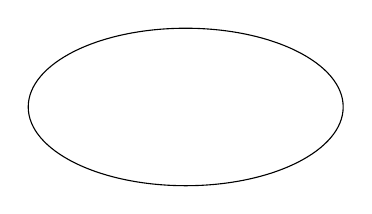
\begin{tikzpicture}
        \draw (1,1) ellipse (2 and 1);
    \end{tikzpicture}    
    \caption{椭圆}
    \label{f2}
\end{figure}